\documentclass[10pt,twoside,a4paper,openright]{report}
\usepackage[Bjornstrup]{fncychap}
% enforce latex compiler to interpret files as utf8 encoded
\usepackage[utf8]{inputenc}
% Make latex understand and use the typographic
% rules of the language used in the document.
\usepackage[danish,english]{babel}
% Use the vector font Latin Modern which is going
% to be the default font in latex in the future.
\usepackage{lmodern}
% Choose the font encoding
\usepackage[T1]{fontenc}

\usepackage{float}
\restylefloat{table}
% load a colour package
\usepackage[table,xcdraw]{xcolor}
%\usepackage{xcolor}
\definecolor{aaublue}{RGB}{33,26,82}% dark blue
% The standard graphics inclusion package
\usepackage{graphicx}
% Set up how figure and table captions are displayed
\usepackage{caption}
\captionsetup{%
  font=footnotesize,% set font size to footnotesize
  labelfont=bf % bold label (e.g., Figure 3.2) font
}
% Make the standard latex tables look so much better
\usepackage{array,booktabs}
% Enable the use of frames around, e.g., theorems
% The framed package is used in the example environment
\usepackage{framed}
%% source code listing.
\usepackage{listings}
% Defines new environments such as equation,
% align and split 
\usepackage{amsmath}
% Adds new math symbols
\usepackage{amssymb}
% Use theorems in your document
% The ntheorem package is also used for the example environment
% When using thmmarks, amsmath must be an option as well. Otherwise \eqref doesn't work anymore.
\usepackage[framed,amsmath,thmmarks]{ntheorem}
% Change the headers and footers
\usepackage{fancyhdr}
% Enable arithmetics with length. Useful when
% typesetting the layout.
\usepackage{calc}

%cross sign
\usepackage{bbding}

% Add the \citep{key} command which display a
% reference as [author, year]
%\usepackage[square]{natbib}
% Appearance of the bibliography
\bibliographystyle{plain}

%%%%%%%%%%%%%%%%%%%%%%%%%%%%%%%%%%%%%%%%%%%%%%%%
% Misc
%%%%%%%%%%%%%%%%%%%%%%%%%%%%%%%%%%%%%%%%%%%%%%%%%
% for multicolumn itemize and enumations
\usepackage{multicol}
% Add bibliography and index to the table of
% contents
\usepackage[nottoc]{tocbibind}
% Add the command \pageref{LastPage} which refers to the
% page number of the last page
% package required in order to use LastPage
\usepackage{lastpage}

\usepackage[
%  disable, %turn off todonotes
  colorinlistoftodos, %enable a coloured square in the list of todos
  textwidth=\marginparwidth, %set the width of the todonotes
  textsize=scriptsize, %size of the text in the todonotes
  ]{todonotes}

% enable english st, nd, rd, th to numbers
  \usepackage{nth}
% Enable hyperlinks and insert info into the pdf
% file. Hypperref should be loaded as one of the 
% last packages
\usepackage{hyperref}
\hypersetup{%
	pdfpagelabels=true,%
	plainpages=false,%
	pdfauthor={Author (s)},%
	pdftitle={Title},%
	pdfsubject={Subject},%
	bookmarksnumbered=true,%
	colorlinks,%
	citecolor=aaublue,%
	filecolor=aaublue,%
	linkcolor=aaublue,% you should probably change this to black before printing
	urlcolor=aaublue,%
	pdfstartview=FitH%
}

% Enable printing of section/chapter name instead of number.
% Requires use of \nameref{<label>} instead of \ref{<label>}.
\usepackage{nameref}

% Dont know what this does, but was required for formatting tables
% as specific way
\usepackage{rotating}
\usepackage{pifont}
\newcommand*\rot{\rotatebox{90}}
\newcommand*\tilt{\rotatebox{70}}
\newcommand*\OK{\ding{51}}

% setup code listings to sane defaults
\lstset{frame=single,
    keepspaces=true,
    keywordstyle=\color{blue},
    numbers=left,
    captionpos=b,
    breakatwhitespace=true,
    breaklines=true,
    tabsize=2,
    basicstyle=\ttfamily\footnotesize}

% used to include eps files
\usepackage{epstopdf}

% This package allows changing of counters in latex
% We use it to use continuous numbering of chapters across parts.
\usepackage{chngcntr}

% Sort of replaces hyperref
\usepackage{bookmark}

% Allows nested figures
\usepackage{subcaption}

%Anders COMMAND
\newcommand{\todoanders}[2][ ]
{
  \ifthenelse{\equal{#1}{inline}}
    {\todo[inline, size=\small, color=blue!40]{\textbf{Anders:} #2}}
    {{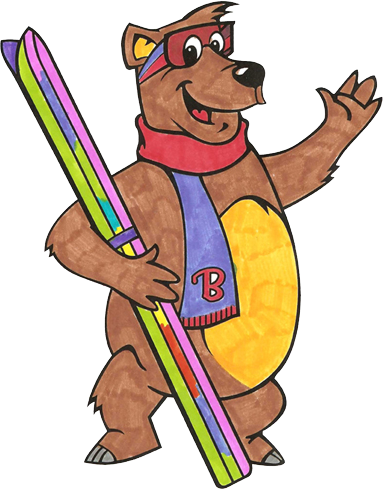
\includegraphics[height=2ex]{setup/Comments/anders}} \todo[size=\small, color=blue!40]{\textbf{Anders:} #2}}
}


%Benjamin COMMAND
\newcommand{\todobenjamin}[2][ ]
{
  \ifthenelse{\equal{#1}{inline}}
    {\todo[inline, size=\small, color=blue!40]{\textbf{Benjamin:} #2}}
    {{
\includegraphics[height=2ex]{setup/Comments/benjamin}} \todo[size=\small, color=yellow!40]{\textbf{Benjamin:} #2}}
}

%Daniel COMMAND
\newcommand{\tododaniel}[2][ ]
{
  \ifthenelse{\equal{#1}{inline}}
    {\todo[inline, size=\small, color=blue!40]{\textbf{Daniel:} #2}}
    {{
\includegraphics[height=2ex]{setup/Comments/daniel}} \todo[size=\small, color=green!40]{\textbf{Daniel:} #2}}
}


%Michael COMMAND
\newcommand{\todomichael}[2][ ]
{
  \ifthenelse{\equal{#1}{inline}}
    {\todo[inline, size=\small, color=blue!40]{\textbf{Michael:} #2}}
    {{
\includegraphics[height=2ex]{setup/Comments/michael}} \todo[size=\small, color=orange!40]{\textbf{Michael:} #2}}
}


%Dennis COMMAND
\newcommand{\tododennis}[2][ ]
{
  \ifthenelse{\equal{#1}{inline}}
    {\todo[inline, size=\small, color=blue!40]{\textbf{Dennis:} #2}}
    {{
\includegraphics[height=2ex]{setup/Comments/dennis}} \todo[size=\small, color=purple!40]{\textbf{Dennis:} #2}}
}

%Kasper COMMAND
\newcommand{\todokasper}[2][ ]
{
  \ifthenelse{\equal{#1}{inline}}
    {\todo[inline, size=\small, color=blue!40]{\textbf{Kasper:} #2}}
    {{
\includegraphics[height=2ex]{setup/Comments/kasper}} \todo[size=\small, color=pink!40]{\textbf{Kasper:} #2}}
}

%Brian COMMAND
\newcommand{\todobrian}[2][ ]
{
  \ifthenelse{\equal{#1}{inline}}
    {\todo[inline, size=\small, color=blue!40]{\textbf{Brian:} #2}}
    {{
\includegraphics[height=2ex]{setup/Comments/brian}} \todo[size=\small, color=red!40]{\textbf{Brian:} #2}}
}


